\chapter{คู่มือปฏิบัติการจุลชีววิทยาการเกษตรมาตรฐาน}
\label{ch:lab_manual}

\begin{keyconcept}[แนวคิดสำคัญของบทที่ 11]
การเรียนรู้และวิจัยทางจุลชีววิทยาการเกษตรระดับอุดมศึกษาจะสมบูรณ์ได้ต้องอาศัยการฝึกฝนทักษะปฏิบัติการ (Hands-on Laboratory Skills) อย่างเป็นระบบ บทนี้รวบรวมระเบียบวิธีปฏิบัติการทดลองมาตรฐาน 8 ปฏิบัติการ ครอบคลุมตั้งแต่การศึกษานิเวศวิทยาจุลินทรีย์ดินด้วยคอลัมน์วิโนกราดสกี การแยกและคัดเลือกจุลินทรีย์ส่งเสริมการเจริญเติบโตของพืช (PGPR) และราปฏิปักษ์ การตรวจสอบคุณภาพปุ๋ยชีวภาพตามเกณฑ์กฎหมาย ตลอดจนเทคนิคอณูชีววิทยาขั้นสูง (การสกัด Soil Metagenomic DNA, การตรวจวินิจฉัยเชื้อก่อโรคด้วย PCR และการประเมินพื้นที่โรคพืชด้วยวิทัศน์คอมพิวเตอร์) เพื่อให้นักศึกษาสามารถบูรณาการทฤษฎีสู่การปฏิบัติจริงในระดับมืออาชีพ
\end{keyconcept}

\begin{figure}[ht]
    \centering
    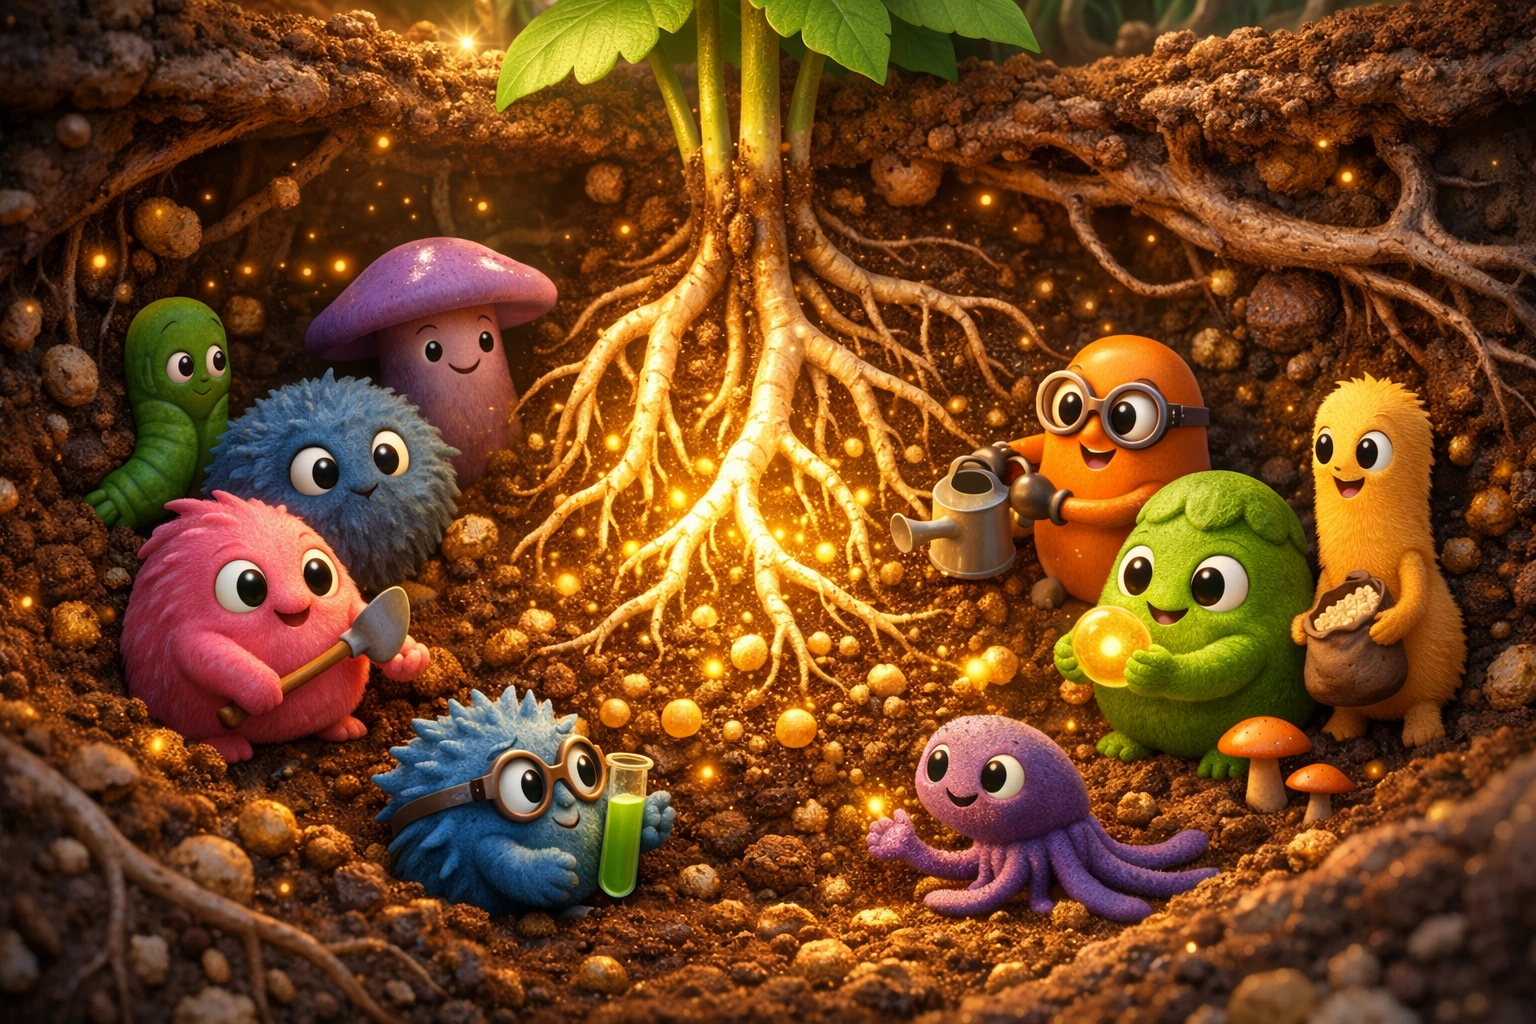
\includegraphics[width=0.85\textwidth]{assets/ch11_lab_manual.png}
    \caption{ภาพรวมการปฏิบัติการจุลชีววิทยาการเกษตรมาตรฐาน แสดงการทำงานภายใต้ตู้ถ่ายเชื้อปลอดเชื้อ (Laminar Airflow Cabinet) การเพาะเลี้ยงเชื้อบนจานอาหารเลี้ยงเชื้อสังเคราะห์ การย้อมสีส่องกล้องจุลทรรศน์ และการวิเคราะห์สารพันธุกรรมด้วยเครื่องเพิ่มปริมาณสารพันธุกรรม PCR}
    \label{fig:ch11_lab_overview}
\end{figure}

\section*{วัตถุประสงค์การเรียนรู้ประจำบท}
เมื่อศึกษาและฝึกปฏิบัติการในบทนี้จบแล้ว นักศึกษาสามารถ:
\begin{enumerate}
    \item ปฏิบัติตนตามระเบียบความปลอดภัยในห้องปฏิบัติการจุลชีววิทยาการเกษตร (Biosafety Level 1 และ 2) ได้อย่างถูกต้อง
    \item ดำเนินการแยก คัดเลือก และทดสอบประสิทธิภาพของ \organism{Rhizobium}, แบคทีเรียละลายฟอสเฟต (PSI), และราปฏิปักษ์ \organism{Trichoderma} (PIRG)
    \item ย้อมสีและประเมินเปอร์เซ็นต์การเข้าอยู่อาศัยของเชื้อราอาร์บัสคูลาร์ไมคอร์ไรซา (AMF) ในรากพืชด้วยวิธี Gridline Intersect Method
    \item ตรวจสอบคุณภาพปุ๋ยชีวภาพทั้งปริมาณเซลล์มีชีวิต (CFU/g) และการตรวจหาเชื้อปนเปื้อนตามมาตรฐาน พ.ร.บ. ปุ๋ย
    \item สกัด DNA จุลินทรีย์จากดิน ตรวจวัดความบริสุทธิ์ด้วยค่า $A_{260}/A_{280}$ และทำปฏิกิริยา PCR สำหรับการตรวจวินิจฉัยเชื้อโรคพืช
\end{enumerate}

\begin{arinteraction}[นวัตกรรมตำราเรียนดิจิทัล: ระบบ AR 3D Interactive ArUco Book]
คู่มือปฏิบัติการในบทนี้ได้รับการออกแบบบูรณาการร่วมกับระบบความจริงเสริม (WebAR) แบบโต้ตอบ 60 FPS ผู้เรียนสามารถใช้สมาร์ตโฟนสแกนรหัส \textbf{ArUco Marker (DICT\_6X6\_250)} ที่ปรากฏคู่กับแต่ละปฏิบัติการ เพื่อเปิดดูแบบจำลอง 3 มิติเสมือนจริง อุปกรณ์แล็บจำลอง และโครงสร้างชีวโมเลกุลสามมิติ (PDB Structures) แบบหมุนสำรวจ $360^\circ$ ได้ทันทีผ่านเบราว์เซอร์โดยไม่ต้องติดตั้งโปรแกรมเพิ่มเติม

\vspace{1mm}
\noindent\textbf{ลิงก์เข้าใช้งานระบบ WebAR:} \url{http://localhost/ar_3d_aruco_book/} หรือใช้ร่วมกับแผ่นพิมพ์การ์ดมาร์กเกอร์ตัดประกอบในไฟล์ \texttt{ar\_markers\_sheet\_A4.pdf}
\end{arinteraction}

\section{ระเบียบความปลอดภัยและเทคนิคปลอดเชื้อ (Aseptic Technique)}

ห้องปฏิบัติการจุลชีววิทยาการเกษตรจัดอยู่ในระดับ \textbf{Biosafety Level 1 (BSL-1)} ถึง \textbf{Biosafety Level 2 (BSL-2)}\index{Biosafety Level (BSL)} นักศึกษาต้องปฏิบัติตามกฎความปลอดภัยอย่างเคร่งครัด:
\begin{enumerate}
    \item \textbf{การเตรียมตัวและการแต่งกาย:} สวมเสื้อกาวน์แขนยาว ถุงมือไนไตรล์ แว่นตานิรภัย และรองเท้าหุ้มส้นตลอดเวลา ห้ามรับประทานอาหาร ดื่มน้ำ หรือสัมผัสใบหน้าระหว่างปฏิบัติการ
    \item \textbf{เทคนิคปลอดเชื้อ (Aseptic Technique):\index{เทคนิคปลอดเชื้อ (Aseptic Technique)}} ทำความสะอาดโต๊ะปฏิบัติการด้วยแอลกอฮอล์ $70\% \text{ (v/v)}$ ก่อนและหลังการทดลอง จุดตะเกียงแอลกอฮอล์เพื่อสร้างรัศมีปลอดเชื้อ $10 - 15\text{ cm}$ หรือปฏิบัติงานในตู้ถ่ายเชื้อปลอดเชื้อ (Laminar Airflow Cabinet) ลนไฟห่วงเพลทเชื้อ (Inoculating loop) จนแดงและปล่อยให้เย็นก่อนสัมผัสโคโลนี
    \item \textbf{การนึ่งฆ่าเชื้อ (Autoclaving):\index{การนึ่งฆ่าเชื้อด้วยไอน้ำ (Autoclaving)}} อาหารเลี้ยงเชื้อ อุปกรณ์แก้ว และของเสียชีวภาพ ต้องผ่านการนึ่งฆ่าเชื้อด้วยไอน้ำอัดความดันที่อุณหภูมิ \textbf{$121^\circ\text{C}$ ความดัน 15 ปอนด์ต่อตารางนิ้ว (psi) เป็นเวลาไม่น้อยกว่า 15--20 นาที}
    \item \textbf{การกำจัดขยะอันตรายชีวภาพ (Biohazard Waste):} ทิ้งจานเพาะเชื้อ ปิเปตทิป และหลอดทดลองที่ปนเปื้อนเชื้อในถังขยะชีวภาพสีแดงเพื่อนำไปผ่านการ Autoclave ก่อนทิ้งสู่ภายนอก
\end{enumerate}

\begin{figure}[ht]
\centering
\resizebox{0.96\textwidth}{!}{
\begin{tikzpicture}[
    level 1/.style={sibling distance=4.5cm, level distance=1.6cm},
    level 2/.style={sibling distance=3.2cm, level distance=1.8cm},
    level 3/.style={sibling distance=2.2cm, level distance=2.0cm},
    root/.style={draw=navyprimary, fill=navyprimary!10, rounded corners=4pt, font=\bfseries\small, text width=3.8cm, align=center, line width=1pt},
    group/.style={draw=forestgreen, fill=forestgreen!10, rounded corners=4pt, font=\bfseries\footnotesize, text width=2.8cm, align=center, line width=0.8pt},
    charact/.style={draw=earthbrown, fill=earthbrown!10, rounded corners=3pt, font=\scriptsize, text width=2.6cm, align=center},
    outcome/.style={draw=navyprimary, fill=amber!20, rounded corners=3pt, font=\bfseries\scriptsize, text width=2.4cm, align=center, line width=0.8pt},
    edge from parent/.style={draw=navyprimary!80, line width=0.8pt, ->, >=Stealth}
]
    \node [root] {การจำแนกจุลินทรีย์การเกษตร\\เบื้องต้นในห้องปฏิบัติการ}
        child {
            node [group] {แบคทีเรียแกรมบวก\\(Gram-Positive)}
            child {
                node [charact] {แท่ง สร้างสปอร์\\Catalase (+)}
                child { node [outcome] {\organism{Bacillus} spp.\\(PGPR / ปุ๋ยชีวภาพ)} }
            }
            child {
                node [charact] {เส้นใยแตกแขนง\\กลิ่นไอดิน (Geosmin)}
                child { node [outcome] {\organism{Streptomyces} spp.\\(ปฏิปักษ์/ย่อยสลาย)} }
            }
        }
        child {
            node [group] {แบคทีเรียแกรมลบ\\(Gram-Negative)}
            child {
                node [charact] {แท่ง สร้างเม็ดสีเรืองแสง\\บนอาหาร King's B}
                child { node [outcome] {\organism{Pseudomonas} spp.\\(ละลายฟอสเฟต/ไซเดอโรฟอร์)} }
            }
            child {
                node [charact] {แยกจากปมรากถั่ว\\อาหาร YEMA+CR ไม่ดูดสี}
                child { node [outcome] {\organism{Rhizobium} spp.\\(ตรึงไนโตรเจนพึ่งพา)} }
            }
        }
        child {
            node [group] {เชื้อราและโอโอไมซีต\\(Fungi / Oomycetes)}
            child {
                node [charact] {โตเร็ว สปอร์สีเขียวเข้ม\\สร้างก้านสปอร์แตกแขนง}
                child { node [outcome] {\organism{Trichoderma} spp.\\(ราปฏิปักษ์ควบคุมโรค)} }
            }
            child {
                node [charact] {เส้นใยไม่มีผนังกั้น\\สปอร์แรนเจียมคล้ายเลมอน}
                child { node [outcome] {\organism{Phytophthora} spp.\\(เชื้อราโรครากเน่า)} }
            }
        };
\end{tikzpicture}
}
\caption{ต้นไม้การตัดสินใจ (Decision Tree) สำหรับการตรวจวินิจฉัยและจำแนกกลุ่มจุลินทรีย์การเกษตรสำคัญในห้องปฏิบัติการ}
\label{fig:microbe_diagnostic_tree}
\end{figure}

\section{ปฏิบัติการที่ 1: การสร้างและศึกษานิเวศวิทยา Winogradsky Column}

\textbf{วัตถุประสงค์:} เพื่อศึกษานิเวศวิทยาจุลินทรีย์ดิน การแบ่งชั้นตามความเข้มข้นของออกซิเจนและซัลไฟด์ และการเติบโตของจุลินทรีย์สังเคราะห์แสง

\begin{labprotocol}[ขั้นตอนการทดลอง Winogradsky Column]
\textbf{วัสดุและอุปกรณ์:} กระบอกตวงพลาสติกหรือขวดแก้วใสทรงสูง (ขนาด $500 - 1,000\text{ mL}$), โคลนจากท้องร่องสวนหรือก้นหนองน้ำ, กระดาษกรองสับละเอียด $5\text{ g}$ (แหล่งคาร์บอนเซลลูโลส), แคลเซียมซัลเฟต ($CaSO_4$) $5\text{ g}$, แคลเซียมคาร์บอเนต ($CaCO_3$) $5\text{ g}$, แรปพลาสติกใส, โคมไฟส่องสว่างหลอดไส้ 40--60 วัตต์

\textbf{ขั้นตอนการทำปฏิบัติการ:}
\begin{enumerate}
    \item นำดินโคลนมาผสมกับ $CaSO_4, CaCO_3$ และเศษกระดาษกรองสับให้เข้ากันเป็นเนื้อเดียว
    \item บรรจุส่วนผสมดินโคลนลงในกระบอกแก้วให้สูงประมาณ $1/3$ เคาะไล่ฟองอากาศให้แน่น
    \item ตักดินโคลนที่ไม่ผสมสารเคมีเติมลงไปต่อจนสูงถึง $2/3$ ของกระบอก
    \item เติมน้ำจากแหล่งน้ำธรรมชาติลงไปจนเหลือช่องว่างอากาศด้านบนประมาณ $2 - 3\text{ cm}$
    \item ปิดปากกระบอกด้วยแรปพลาสติกใสและรัดหนังยางให้แน่นเพื่อป้องกันน้ำระเหย
    \item วางกระบอกตวงไว้ใกล้หน้าต่างหรือส่องด้วยโคมไฟห่างประมาณ 20 ซม. บ่มไว้เป็นเวลา 4--8 สัปดาห์
    \item สังเกตการแบ่งชั้นสีของจุลินทรีย์: ชั้นล่างสุดสีดำ (\organism{Desulfovibrio}), ชั้นสีเขียวเข้ม (Green sulfur bacteria: \organism{Chlorobium}), ชั้นสีแดงอมม่วง (Purple sulfur bacteria: \organism{Chromatium}), และชั้นผิวน้ำสีเขียวสว่าง (Algae และ Cyanobacteria)
\end{enumerate}
\end{labprotocol}

\begin{arinteraction}[AR 3D Interactive Simulation: Winogradsky Eco-Column (ArUco ID: 0)]
\begin{minipage}[c]{0.26\textwidth}
    \centering
    
\includegraphics[width=\linewidth]{assets/aruco/aruco_id_0.png}
\end{minipage}\hfill
\begin{minipage}[c]{0.70\textwidth}
    \small
    \textbf{ส่องด้วยสมาร์ตโฟนผ่าน WebAR เพื่อดูแบบจำลอง 3 มิติเสมือนจริง}\\
    \textbf{แบบจำลอง 3D:} Winogradsky Eco-Column หลอดทดลอง 4 ชั้นนิเวศจุลินทรีย์ดิน\\
    \textbf{ฟังก์ชันเชิงโต้ตอบ:} หมุนสำรวจการแบ่งชั้นจุลินทรีย์ (\organism{Desulfovibrio}, \organism{Chlorobium}, \organism{Chromatium}, \organism{Cyanobacteria}) และการไล่ระดับความเข้มข้นสัมพัทธ์ของก๊าซ $O_2$ และ $H_2S$ แบบเรียลไทม์ 60 FPS
\end{minipage}
\end{arinteraction}

\section{ปฏิบัติการที่ 2: การแยกและทดสอบประสิทธิภาพ Rhizobium จากปมรากถั่ว}

\textbf{วัตถุประสงค์:} เพื่อแยกเชื้อบริสุทธิ์ของ \organism{Rhizobium}\index{Rhizobium@\textit{Rhizobium}} และประเมินความมีชีวิตของโปรตีนเลกเฮโมโกลบินในปมราก

\begin{labprotocol}[ขั้นตอนการแยกเชื้อ Rhizobium]
\textbf{วัสดุและอุปกรณ์:} ปมรากถั่วสดที่มีสีชมพูเรื่อด้านใน, เอทานอล 70\%, สารละลายโซเดียมไฮโปคลอไรต์ 1\%, น้ำกลั่นนึ่งฆ่าเชื้อ, อาหาร Yeast Extract Mannitol Agar ผสม Congo Red (YEMA-CR)\index{อาหารเลี้ยงเชื้อ YEMA (Yeast Extract Mannitol Agar)}, แท่งแก้วบดปลอดเชื้อ

\textbf{ขั้นตอนการทำปฏิบัติการ:}
\begin{enumerate}
    \item เลือกปมรากที่สมบูรณ์ ผ่าครึ่งเพื่อยืนยันสีชมพูของเลกเฮโมโกลบิน (Active nitrogen fixation)
    \item จุ่มปมรากในเอทานอล 70\% นาน 10 วินาที จากนั้นย้ายลงในสารละลายไฮโปคลอไรต์ 1\% นาน 3 นาที เพื่อฟอกฆ่าเชื้อที่ผิว (Surface sterilization)
    \item ล้างน้ำกลั่นนึ่งฆ่าเชื้อ 5 ครั้งเพื่อกำจัดสารฟอกขาวตกค้าง
    \item ใส่ปมรากลงในหลอดทดลอง เติมน้ำกลั่นปลอดเชื้อ $0.2\text{ mL}$ แล้วบดด้วยแท่งแก้วจนละเอียด
    \item แตะสารแขวนลอยนำมาเกลี่ยแบบ Streak plate บนอาหาร YEMA-CR บ่มที่ $28^\circ\text{C}$ นาน 3--5 วัน
    \item ตรวจดูลักษณะโคโลนี: \organism{Rhizobium} จะมีลักษณะกลมนูน เมือกเหนียวขุ่น สีขาวหรือชมพูอ่อนมาก โดย \textbf{ไม่ดูดซับสีย้อมคองโกเรด} เข้าสู่เซลล์ (ต่างจากแบคทีเรียปนเปื้อนที่ติดสีแดงเข้ม)
\end{enumerate}
\end{labprotocol}

\begin{arinteraction}[AR 3D Interactive Simulation: Rhizobium \& Leghemoglobin 1GDJ (ArUco ID: 1)]
\begin{minipage}[c]{0.26\textwidth}
    \centering
    
\includegraphics[width=\linewidth]{assets/aruco/aruco_id_1.png}
\end{minipage}\hfill
\begin{minipage}[c]{0.70\textwidth}
    \small
    \textbf{ส่องด้วยสมาร์ตโฟนผ่าน WebAR เพื่อดูแบบจำลอง 3 มิติเสมือนจริง}\\
    \textbf{แบบจำลอง 3D:} โครงสร้างปมรากถั่วผ่าซีก และโครงสร้างโมเลกุล 3D โปรตีนเลกเฮโมโกลบิน (\textit{Leghemoglobin}, PDB ID: \texttt{1GDJ})\\
    \textbf{ฟังก์ชันเชิงโต้ตอบ:} สำรวจโครงข่ายฮีมพ็อกเก็ต (Heme pocket) ดักจับโมเลกุลออกซิเจน เพื่อรักษาสภาวะไม่ใช้ออกซิเจนแก่เอนไซม์ไนโตรจีเนสในแบคทีรอยด์
\end{minipage}
\end{arinteraction}

\section{ปฏิบัติการที่ 3: การคัดเลือกจุลินทรีย์ละลายฟอสเฟต (PSI)}

\textbf{วัตถุประสงค์:} เพื่อคัดแยกจุลินทรีย์ที่มีศักยภาพละลายฟอสเฟตและคำนวณดัชนี Phosphate Solubilization Index (PSI)\index{Phosphate Solubilization Index (PSI)}

\begin{labprotocol}[ขั้นตอนการวัดค่าดัชนี PSI บนอาหาร Pikovskaya]
\textbf{วัสดุและอุปกรณ์:} อาหารแข็ง Pikovskaya's Agar\index{อาหารเลี้ยงเชื้อ Pikovskaya} (มีตะกอนแคลเซียมฟอสเฟต $Ca_3(PO_4)_2$ สีขาวขุ่น), หัวเชื้อจุลินทรีย์ดินตัวอย่าง, เวอร์เนียคาลิปเปอร์

\textbf{ขั้นตอนการทำปฏิบัติการ:}
\begin{enumerate}
    \item จุดหัวเชื้อ (Spot inoculation) ปริมาตร $10\mu\text{L}$ ลงบนกึ่งกลางจานอาหาร Pikovskaya จำนวน 3 ซ้ำ
    \item บ่มที่อุณหภูมิ $30^\circ\text{C}$ เป็นเวลา 5 วัน (แบคทีเรีย) หรือ 7 วัน (เชื้อรา)
    \item วัดเส้นผ่านศูนย์กลางของโคโลนี ($d_c$) และเส้นผ่านศูนย์กลางของวงใส (Clear zone diameter: $d_z$) ด้วยเวอร์เนียคาลิปเปอร์
    \item คำนวณค่าดัชนีการละลายฟอสเฟต:
    \begin{equation}
    \text{PSI} = \frac{d_z}{d_c}
    \end{equation}
\end{enumerate}
เกณฑ์การประเมิน: ค่า $\text{PSI} \ge 2.0$ จัดเป็นจุลินทรีย์ที่มีประสิทธิภาพสูงมากในการปลดปล่อยฟอสฟอรัส
\end{labprotocol}

\begin{arinteraction}[AR 3D Interactive Simulation: Phosphate Solubilizer PSI Assay (ArUco ID: 2)]
\begin{minipage}[c]{0.26\textwidth}
    \centering
    
\includegraphics[width=\linewidth]{assets/aruco/aruco_id_2.png}
\end{minipage}\hfill
\begin{minipage}[c]{0.70\textwidth}
    \small
    \textbf{ส่องด้วยสมาร์ตโฟนผ่าน WebAR เพื่อดูแบบจำลอง 3 มิติเสมือนจริง}\\
    \textbf{แบบจำลอง 3D:} จานเพาะเชื้อ Pikovskaya Agar แสดงโคโลนีและวงใสละลายหินฟอสเฟต (Clear Zone) พร้อมเวอร์เนียคาลิปเปอร์จำลอง\\
    \textbf{ฟังก์ชันเชิงโต้ตอบ:} ปรับเลื่อนแถบเวอร์เนียวัดขนาดเส้นผ่านศูนย์กลาง $d_z$ และ $d_c$ พร้อมระบบคำนวณและประเมินค่าดัชนี $\text{PSI} = d_z / d_c$ โดยอัตโนมัติ
\end{minipage}
\end{arinteraction}

\section{ปฏิบัติการที่ 4: การทดสอบกิจกรรมปฏิปักษ์ของ Trichoderma (PIRG)}

\textbf{วัตถุประสงค์:} เพื่อประเมินความสามารถในการยับยั้งเชื้อราก่อโรคพืชของ \organism{Trichoderma harzianum} ด้วยเทคนิค Dual Culture\index{Dual Culture Assay}

\begin{labprotocol}[ขั้นตอนการทดสอบ Dual Culture Confrontation Assay]
\textbf{วัสดุและอุปกรณ์:} อาหาร Potato Dextrose Agar (PDA), จานเลี้ยงเชื้อ \organism{Trichoderma harzianum} อายุ 5 วัน, จานเลี้ยงเชื้อราก่อโรค (เช่น \organism{Fusarium oxysporum} หรือ \organism{Colletotrichum} sp.), Cork borer ขนาดเส้นผ่านศูนย์กลาง $5\text{ mm}$

\textbf{ขั้นตอนการทำปฏิบัติการ:}
\begin{enumerate}
    \item ใช้ Cork borer เจาะชิ้นวุ้นขอบโคโลนีราก่อโรค วางลงบนจานอาหาร PDA ห่างจากขอบจาน $1.5\text{ cm}$
    \item เจาะชิ้นวุ้นราปฏิปักษ์ \organism{Trichoderma} วางตรงข้ามกันห่างจากขอบอีกด้าน $1.5\text{ cm}$ (ระยะห่างระหว่างชิ้นวุ้นทั้งสองประมาณ $5.0\text{ cm}$)
    \item ทำจานควบคุม (Control plate) โดยวางชิ้นวุ้นราก่อโรคเพียงอย่างเดียว
    \item บ่มที่อุณหภูมิห้อง ($25-28^\circ\text{C}$) ตรวจวัดรัศมีการเจริญของเชื้อราก่อโรคเข้าหาเชื้อปฏิปักษ์ ($R_2$) และวัดรัศมีเชื้อราก่อโรคในจานควบคุม ($R_1$) เมื่อจานควบคุมเจริญเกือบเต็มจาน (ประมาณวันที่ 5--7)
    \item คำนวณเปอร์เซ็นต์การยับยั้งการเจริญของรัศมีเส้นใย:
    \begin{equation}
    \text{PIRG (\%)} = \frac{R_1 - R_2}{R_1} \times 100
    \end{equation}
\end{enumerate}
\end{labprotocol}

\begin{arinteraction}[AR 3D Interactive Simulation: Trichoderma Confrontation \& Chitinase 1CTN (ArUco ID: 3)]
\begin{minipage}[c]{0.26\textwidth}
    \centering
    
\includegraphics[width=\linewidth]{assets/aruco/aruco_id_3.png}
\end{minipage}\hfill
\begin{minipage}[c]{0.70\textwidth}
    \small
    \textbf{ส่องด้วยสมาร์ตโฟนผ่าน WebAR เพื่อดูแบบจำลอง 3 มิติเสมือนจริง}\\
    \textbf{แบบจำลอง 3D:} จานประจันหน้า Dual Culture (\organism{Trichoderma} ปะทะ \organism{Fusarium}) และโมเลกุลเอนไซม์ไคติเนส (\textit{Chitinase}, PDB ID: \texttt{1CTN})\\
    \textbf{ฟังก์ชันเชิงโต้ตอบ:} จำลองกลไก Mycoparasitism การแทงเส้นใยพันรัด ปลดปล่อยเอนไซม์ย่อยสลายผนังเซลล์ราโรคพืช และคำนวณค่า PIRG (\%)
\end{minipage}
\end{arinteraction}

\section{ปฏิบัติการที่ 5: การย้อมสีและตรวจหาเชื้อราไมคอร์ไรซาในรากพืช}

\textbf{วัตถุประสงค์:} เพื่อเตรียมสไลด์รากพืช ย้อมสีโครงสร้างอาร์บัสคูลและเวสิเคิลของ AMF และประเมินเปอร์เซ็นต์การเข้าอยู่อาศัยในราก

\begin{labprotocol}[การย้อมสีรากด้วยวิธี Trypan Blue และวิธี Gridline Intersect]
\textbf{วัสดุและอุปกรณ์:} รากฝอยพืชสด (ข้าวโพดหรือหญ้า), สารละลายโพแทสเซียมไฮดรอกไซด์ (KOH) 10\%, กรดไฮโดรคลอริก (HCl) 1\%, สีย้อม Trypan Blue 0.05\% ในแลกโตกลีเซอรอล\index{การย้อมสีย้อม Trypan Blue}, จานเพาะเชื้อกริดตาราง (Gridline dish), กล้องจุลทรรศน์สเตอริโอและกล้องเลนส์ประกอบ

\textbf{ขั้นตอนการทำปฏิบัติการ:}
\begin{enumerate}
    \item ล้างรากพืชให้สะอาด ตัดเป็นท่อนยาวประมาณ $1\text{ cm}$
    \item แช่รากในสารละลาย KOH 10\% ในอ่างน้ำร้อน ($90^\circ\text{C}$) นาน 30--45 นาที เพื่อฟอกล้างไซโตพลาสซึมของเซลล์พืช (Root Clearing)
    \item ล้างด้วยน้ำสะอาด แล้วแช่ในสารละลาย HCl 1\% นาน 5 นาที เพื่อปรับสภาพความเป็นกรด
    \item ย้ายรากลงแช่ในสีย้อม Trypan Blue 0.05\% ในอ่างน้ำร้อน ($90^\circ\text{C}$) นาน 15 นาที
    \item ล้างสีส่วนเกินออกด้วยสารละลายแลกโตกลีเซอรอลบริสุทธิ์
    \item นำชิ้นราก 50--100 ชิ้นมาเรียงบนจานแก้วที่มีเส้นกริดตารางขนาด $0.5 \times 0.5\text{ cm}$ ส่องตรวจจุดตัดระหว่างเส้นกริดกับชิ้นราก (Gridline Intersect Method)\index{Gridline Intersect Method}
    \item ตรวจนับจุดตัดที่มีโครงสร้าง AMF (Arbuscules, Vesicles, Hyphae) และจุดตัดทั้งหมด
    \begin{equation}
    \% \text{ AMF Colonization} = \frac{\text{จำนวนจุดตัดที่พบโครงสร้าง AMF}}{\text{จำนวนจุดตัดของรากทั้งหมด}} \times 100
    \end{equation}
\end{enumerate}
\end{labprotocol}

\begin{arinteraction}[AR 3D Interactive Simulation: AMF Root Colonization \& Gridline (ArUco ID: 4)]
\begin{minipage}[c]{0.26\textwidth}
    \centering
    
\includegraphics[width=\linewidth]{assets/aruco/aruco_id_4.png}
\end{minipage}\hfill
\begin{minipage}[c]{0.70\textwidth}
    \small
    \textbf{ส่องด้วยสมาร์ตโฟนผ่าน WebAR เพื่อดูแบบจำลอง 3 มิติเสมือนจริง}\\
    \textbf{แบบจำลอง 3D:} รากพืชย้อมสี Trypan Blue โครงสร้าง Arbuscule, Vesicle และจานแก้วกริดตาราง\\
    \textbf{ฟังก์ชันเชิงโต้ตอบ:} จำลองการเลื่อนส่องกล้องตรวจจุดตัด Gridline Intersect Method และคำนวณ \% AMF Colonization โดยอัตโนมัติ
\end{minipage}
\end{arinteraction}

\section{ปฏิบัติการที่ 6: การวิเคราะห์คุณภาพปุ๋ยชีวภาพและการตรวจหาเชื้อปนเปื้อน}

\textbf{วัตถุประสงค์:} เพื่อตรวจนับจำนวนเซลล์มีชีวิตของแบคทีเรียปุ๋ยชีวภาพด้วยเทคนิค Serial Dilution Pour Plate และตรวจคัดกรองเชื้อปนเปื้อนตามมาตรฐานกรมวิชาการเกษตร

\begin{labprotocol}[การตรวจสอบคุณภาพปุ๋ยชีวภาพตามกฎหมาย]
\textbf{วัสดุและอุปกรณ์:} ตัวอย่างปุ๋ยชีวภาพ, สารละลายน้ำเกลือปราศจากเชื้อ 0.85\% NaCl, ปิเปตอัตโนมัติ, อาหารจำเพาะ (YEMA สำหรับ Rhizobium, NA สำหรับนับเชื้อรวม, MacConkey Agar สำหรับตรวจเชื้อกลุ่มโคลิฟอร์ม)\index{อาหาร MacConkey Agar}, ตู้อบเพาะเชื้อ

\textbf{ขั้นตอนการทำปฏิบัติการ:}
\begin{enumerate}
    \item ชั่งตัวอย่างปุ๋ยชีวภาพ $10.0\text{ g}$ ใส่ลงในขวดน้ำเกลือปลอดเชื้อ $90.0\text{ mL}$ เขย่าที่ $180\text{ rpm}$ นาน 30 นาที (ระดับเจือจาง $10^{-1}$)
    \item ดูดสารละลาย $1.0\text{ mL}$ ถ่ายลงในหลอดน้ำเกลือ $9.0\text{ mL}$ ทำการเจือจางแบบสิบเท่าต่อเนื่อง\index{การเจือจางแบบลำดับส่วน (Serial Dilution)}จนถึงระดับ $10^{-8}$
    \item ดูดสารละลายจากระดับเจือจาง $10^{-5}, 10^{-6}, 10^{-7}$ ปริมาตรละ $0.1\text{ mL}$ ลงบนจานอาหารจำเพาะ เกลี่ยด้วยแท่งแก้วสามเหลี่ยม (Spread plate) จานละ 3 ซ้ำ
    \item ดูดสารละลายระดับเจือจาง $10^{-1}$ และ $10^{-2}$ ปริมาตร $0.1\text{ mL}$ เกลี่ยลงบนอาหาร MacConkey Agar เพื่อตรวจหาแบคทีเรียกลุ่มปนเปื้อน \organism{E. coli}
    \item บ่มที่ $30^\circ\text{C}$ นาน 48 ชั่วโมง ตรวจนับจานอาหารที่มีโคโลนีระหว่าง 30--300 โคโลนี คำนวณค่า CFU/g\index{หน่วยนับโคโลนี (CFU)}
    \item ตรวจสอบว่ามีโคโลนีสีชมพูเข้มบน MacConkey Agar หรือไม่ (หากพบแสดงว่าไม่ผ่านเกณฑ์มาตรฐานการปนเปื้อน)
\end{enumerate}
\end{labprotocol}

\begin{arinteraction}[AR 3D Interactive Simulation: Biofertilizer QC \& Dilution (ArUco ID: 5)]
\begin{minipage}[c]{0.26\textwidth}
    \centering
    
\includegraphics[width=\linewidth]{assets/aruco/aruco_id_5.png}
\end{minipage}\hfill
\begin{minipage}[c]{0.70\textwidth}
    \small
    \textbf{ส่องด้วยสมาร์ตโฟนผ่าน WebAR เพื่อดูแบบจำลอง 3 มิติเสมือนจริง}\\
    \textbf{แบบจำลอง 3D:} แร็คหลอดทดลองการเจือจางสิบเท่า ($10^{-1}$ ถึง $10^{-6}$) และจานเพาะเชื้อ MacConkey Agar\\
    \textbf{ฟังก์ชันเชิงโต้ตอบ:} จำลองการตรวจนับโคโลนี CFU/g และการตรวจสอบเชื้อปนเปื้อนกลุ่มโคลิฟอร์มตามมาตรฐาน พ.ร.บ. ปุ๋ย
\end{minipage}
\end{arinteraction}

\section{ปฏิบัติการที่ 7: การสกัด Soil DNA และการตรวจสอบคุณภาพ}

\textbf{วัตถุประสงค์:} เพื่อสกัดสารพันธุกรรม DNA ของไมโครไบโอมดินด้วยเทคนิค Bead-Beating และประเมินความบริสุทธิ์ของ DNA\index{การสกัด DNA จุลินทรีย์ดิน (Soil DNA Extraction)}

\begin{labprotocol}[ขั้นตอนการสกัด Soil Metagenomic DNA]
\textbf{วัสดุและอุปกรณ์:} ตัวอย่างดินไรโซสเฟียร์ $0.25\text{ g}$, ชุดสกัดดิน DNeasy PowerSoil Pro Kit (หรือวิธี Bead-beating CTAB/Phenol-chloroform), เครื่องโฮโมจีไนเซอร์ความเร็วสูง (Bead beater), เครื่องหมุนเหวี่ยงความเย็นสูง, เครื่องสเปกโทรโฟโตมิเตอร์ไมโครวอลุม (Nanodrop)\index{เครื่องสเปกโทรโฟโตมิเตอร์ Nanodrop}, ชุดเจลอิเล็กโทรโฟรซิส

\textbf{ขั้นตอนการทำปฏิบัติการ:}
\begin{enumerate}
    \item ชั่งดิน $0.25\text{ g}$ ใส่ลงในหลอดบรรจุลูกปัดซิลิกา (PowerBead Tube) เติม Lysis Buffer เพื่อช่วยทำลายผนังเซลล์
    \item นำเข้าเครื่อง Bead Beater ปั่นสั่นสะเทือนที่ความเร็ว $6.0\text{ m/s}$ เป็นเวลา 45 วินาที เพื่อทำลายผนังเซลล์แบคทีเรีย แกรมบวก แอคติโนมัยซีส และสปอร์รา
    \item หมุนเหวี่ยงตกตะกอนเศษดินและโปรตีน ดูดสารละลายใสส่วนบนถ่ายลงในหลอดใหม่ เติม Inhibitor Removal Solution เพื่อตกตะกอนกรดฮิวมิก (Humic acids ซึ่งเป็นสารยับยั้งปฏิกิริยา PCR)
    \item ผ่านสารละลายผ่านคอลัมน์ซิลิกา (Silica Spin Column) หมุนเหวี่ยงเพื่อให้ DNA ยึดเกาะกับเยื่อซิลิกา
    \item ล้างคอลัมน์ด้วย Wash Buffer ที่มีเอทานอล 2 ครั้ง หมุนเหวี่ยงเพื่อไล่เอทานอลให้แห้งสนิท
    \item ละลาย DNA ออกจากคอลัมน์ด้วยน้ำปราศจากเอนไซม์นิวคลีเอส (Nuclease-free water) $50\mu\text{L}$
    \item วัดค่าการดูดกลืนแสงที่ความยาวคลื่น $260\text{ nm}$ ($A_{260}$) และ $280\text{ nm}$ ($A_{280}$) ด้วยเครื่อง Nanodrop:
    \begin{itemize}
        \item ความเข้มข้นของ DNA ($\text{ng/}\mu\text{L}$) $= A_{260} \times 50 \times \text{Dilution factor}$
        \item อัตราส่วนความบริสุทธิ์: ค่า $A_{260}/A_{280}$ ที่เหมาะสมควรอยู่ในช่วง \textbf{$1.8 - 2.0$} (หากต่ำกว่า 1.8 แสดงว่ามีโปรตีนหรือกรดฮิวมิกปนเปื้อน)
    \end{itemize}
    \item ตรวจสอบขนาดความสมบูรณ์ของสาย DNA ด้วย Agarose Gel Electrophoresis 1\%\index{เจลอิเล็กโทรโฟริซิส (Agarose Gel Electrophoresis)}
\end{enumerate}
\end{labprotocol}

\begin{arinteraction}[AR 3D Interactive Simulation: Soil DNA Extraction \& B-DNA 1BNA (ArUco ID: 6)]
\begin{minipage}[c]{0.26\textwidth}
    \centering
    
\includegraphics[width=\linewidth]{assets/aruco/aruco_id_6.png}
\end{minipage}\hfill
\begin{minipage}[c]{0.70\textwidth}
    \small
    \textbf{ส่องด้วยสมาร์ตโฟนผ่าน WebAR เพื่อดูแบบจำลอง 3 มิติเสมือนจริง}\\
    \textbf{แบบจำลอง 3D:} หลอด Bead-Beater Lysis, Spin Column, เกลียวคู่ Double-Helix B-DNA (PDB ID: \texttt{1BNA}) และเครื่อง Nanodrop\\
    \textbf{ฟังก์ชันเชิงโต้ตอบ:} หมุนดูโครงสร้างโมเลกุลเกลียวคู่ และกราฟสเปกตรัมดูดกลืนแสง $A_{260}/A_{280}$ ประเมินความบริสุทธิ์ของ DNA
\end{minipage}
\end{arinteraction}

\section{ปฏิบัติการที่ 8: การตรวจวินิจฉัยโรคพืชด้วย PCR และการประเมินภาพด้วย OpenCV}

\textbf{วัตถุประสงค์:} เพื่อเพิ่มปริมาณยีนจำเพาะของเชื้อก่อโรคพืชด้วยปฏิกิริยา Polymerase Chain Reaction (PCR)\index{ปฏิกิริยาลูกโซ่พอลิเมอเรส (PCR)} และประเมินร้อยละพื้นที่แผลบนใบพืชด้วยสคริปต์คอมพิวเตอร์วิทัศน์\index{OpenCV!การคำนวณพื้นที่แผลโรคพืช}

\begin{labprotocol}[ขั้นตอนการทำปฏิกิริยา PCR และการประมวลผลภาพ]
\textbf{ส่วนที่ 1: การทำปฏิกิริยา PCR ตรวจเชื้อ Phytophthora palmivora}
\begin{enumerate}
    \item ผสมสารละลายปฏิกิริยา PCR Master Mix ปริมาตรรวม $25\mu\text{L}$ ต่อหลอด:
    \begin{itemize}
        \item $2\times$ Taq MasterMix (dNTPs, Taq polymerase, Buffer): $12.5\mu\text{L}$
        \item Forward Primer (10 $\mu$M): $1.0\mu\text{L}$
        \item Reverse Primer (10 $\mu$M): $1.0\mu\text{L}$
        \item DNA แม่แบบ (สกัดจากเนื้อเยื่อใบพืชที่เป็นโรค): $2.0\mu\text{L}$ ($20-50\text{ ng}$)
        \item Nuclease-free water: $8.5\mu\text{L}$
    \end{itemize}
    \item โปรแกรมเครื่อง Thermal Cycler:
    \begin{itemize}
        \item Initial Denaturation: $95^\circ\text{C}$ นาน 5 นาที
        \item 35 รอบของ: $95^\circ\text{C}$ (30 วินาที) $\rightarrow 58^\circ\text{C}$ (30 วินาที) $\rightarrow 72^\circ\text{C}$ (45 วินาที)
        \item Final Extension: $72^\circ\text{C}$ นาน 5 นาที
    \end{itemize}
    \item นำผลิตภัณฑ์ PCR ตรวจสอบบนเจลอะกาโรส 1.5\% เทียบกับดีเอ็นเอมาตรฐาน (DNA Ladder 100 bp) สังเกตแถบยีนขนาดจำเพาะ
\end{enumerate}

\textbf{ส่วนที่ 2: การประเมินพื้นที่แผลโรคพืชด้วย Python OpenCV}
\begin{enumerate}
    \item ถ่ายภาพใบพืชที่เป็นโรคบนพื้นหลังสีขาวภายใต้แสงสม่ำเสมอ
    \item รันสคริปต์ Python ในภาคผนวก ข เพื่อแปลงภาพเป็นปริภูมิสี HSV ตัดแยกพิกเซลใบและพิกเซลแผลสะเก็ด
    \item บันทึกค่าร้อยละพื้นที่ความรุนแรงของโรค (DSI) เพื่อนำไปเปรียบเทียบกับผลการตรวจทางอณูชีววิทยา
\end{enumerate}
\end{labprotocol}

\begin{arinteraction}[AR 3D Interactive Simulation: PCR Thermal Cycler \& Vision AI (ArUco ID: 7)]
\begin{minipage}[c]{0.26\textwidth}
    \centering
    
\includegraphics[width=\linewidth]{assets/aruco/aruco_id_7.png}
\end{minipage}\hfill
\begin{minipage}[c]{0.70\textwidth}
    \small
    \textbf{ส่องด้วยสมาร์ตโฟนผ่าน WebAR เพื่อดูแบบจำลอง 3 มิติเสมือนจริง}\\
    \textbf{แบบจำลอง 3D:} เครื่อง Mini PCR Thermal Cycler, ถาดเจลอะกาโรสเรืองแสง UV, เอนไซม์ Taq Polymerase (PDB ID: \texttt{1TAU}) และ OpenCV Bounding Box\\
    \textbf{ฟังก์ชันเชิงโต้ตอบ:} แสดงวงรอบอุณหภูมิ 3 ระดับ การตรวจสอบแถบขนาดดีเอ็นเอ และการตัดตรวจพื้นที่แผลสะเก็ดโรคพืช (DSI \%)
\end{minipage}
\end{arinteraction}

\begin{worked}[ตัวอย่างที่ 11.1 การคำนวณความเข้มข้นและความบริสุทธิ์ของ Soil Metagenomic DNA]
นักศึกษาใช้เครื่อง Nanodrop ตรวจวัดสารละลาย DNA ที่สกัดได้จากดินสวนทุเรียน ได้ค่าการดูดกลืนแสงดังนี้:
$$A_{260} = 0.840 \quad , \quad A_{280} = 0.450 \quad , \quad A_{230} = 0.380$$
จงคำนวณหาความเข้มข้นของ DNA ($\text{ng/}\mu\text{L}$), อัตราส่วนความบริสุทธิ์ $A_{260}/A_{280}$ และ $A_{260}/A_{230}$ พร้อมวิเคราะห์ว่าตัวอย่างนี้สามารถนำไปทำ PCR ได้ทันทีหรือไม่

\textbf{วิธีทำ:}
1. คำนวณความเข้มข้นของ DNA ($1\text{ หน่วย } A_{260} = 50\text{ ng/}\mu\text{L}$ ของ dsDNA):
$$\text{DNA Concentration} = A_{260} \times 50 = 0.840 \times 50 = \mathbf{42.0\text{ ng/}\mu\text{L}}$$

2. คำนวณอัตราส่วนความบริสุทธิ์ $A_{260}/A_{280}$:
$$\frac{A_{260}}{A_{280}} = \frac{0.840}{0.450} \approx \mathbf{1.867}$$

3. คำนวณอัตราส่วนความบริสุทธิ์ $A_{260}/A_{230}$:
$$\frac{A_{260}}{A_{230}} = \frac{0.840}{0.380} \approx \mathbf{2.211}$$

\textbf{บทวิเคราะห์ผลลัพธ์:} ค่า $A_{260}/A_{280} = 1.87$ อยู่ในช่วงมาตรฐานสากล ($1.8 - 2.0$) แสดงว่าปราศจากการปนเปื้อนของโปรตีน และค่า $A_{260}/A_{230} = 2.21$ ($> 2.0$) บ่งชี้ว่าไม่มีกรดฮิวมิกหรือสารทำละลายอินทรีย์หลงเหลืออยู่ ตัวอย่าง DNA นี้มีความบริสุทธิ์ระดับสูงมากและ **พร้อมสำหรับการทำปฏิกิริยา PCR หรือส่งตรวจ NGS ต่อไปได้อย่างสมบูรณ์**
\end{worked}

\begin{worked}[ตัวอย่างที่ 11.2 การประเมินเปอร์เซ็นต์การเข้าอยู่อาศัยของเชื้อรา AMF ในรากข้าวโพด]
จากการส่องตรวจสไลด์รากข้าวโพดย้อมสี Trypan Blue ด้วยวิธี Gridline Intersect Method จำนวนจุดตัดทั้งหมด 120 จุดตัด พบการปรากฏของโครงสร้างเชื้อราไมคอร์ไรซาในรากดังนี้:
\begin{itemize}
    \item พบโครงสร้างเส้นใยและเวสิเคิลร่วมกัน: 45 จุดตัด
    \item พบเฉพาะโครงสร้างอาร์บัสคูล: 30 จุดตัด
    \item พบเฉพาะเส้นใยราภายในเซลล์: 15 จุดตัด
    \item ไม่พบโครงสร้างเชื้อรา: 30 จุดตัด
\end{itemize}
จงคำนวณหาค่าเปอร์เซ็นต์การเข้าอยู่อาศัยของเชื้อราไมคอร์ไรซา (\% AMF Colonization)

\textbf{วิธีทำ:}
1. จำนวนจุดตัดที่ตรวจพบโครงสร้างเชื้อราไมคอร์ไรซา:
$$N_{\text{colonized}} = 45 + 30 + 15 = 90\text{ จุดตัด}$$

2. คำนวณร้อยละการเข้าอยู่อาศัย:
$$\% \text{ AMF Colonization} = \frac{N_{\text{colonized}}}{N_{\text{total}}} \times 100 = \frac{90}{120} \times 100 = \mathbf{75.0\%}$$

\textbf{บทวิเคราะห์ผลลัพธ์:} รากข้าวโพดมีอัตราการเข้าอยู่อาศัยของเชื้อราไมคอร์ไรซาสูงถึง $75.0\%$ ร่วมกับการพบอาร์บัสคูลซึ่งเป็นโครงสร้างแลกเปลี่ยนธาตุอาหาร แสดงว่าพืชมีการพึ่งพาอาศัยทางชีวภาพอย่างสมบูรณ์ ส่งผลให้พืชมีความสามารถในการดูดซับธาตุฟอสฟอรัสในดินแปลงนี้ได้อย่างมีประสิทธิภาพสูง
\end{worked}

\section*{สรุปประจำบท}

คู่มือปฏิบัติการมาตรฐาน 8 การทดลองในบทนี้ทำหน้าที่เป็นแกนกลางเชื่อมโยงทฤษฎีในห้องเรียนสู่งานวิจัยและนวัตกรรมการเกษตรจริง การปฏิบัติตามกฎความปลอดภัยและการรักษาเทคนิคปลอดเชื้อเป็นรากฐานสำคัญของการเพาะเลี้ยงจุลินทรีย์ การเข้าใจหลักการแยกและคัดเลือก \organism{Rhizobium}, แบคทีเรียละลายฟอสเฟต (PSI) และราปฏิปักษ์ \organism{Trichoderma} (PIRG) ตลอดจนการประเมินไมคอร์ไรซา ช่วยให้นักศึกษาสามารถผลิตและควบคุมคุณภาพปุ๋ยชีวภาพได้ตามมาตรฐานกฎหมาย ขณะที่ทักษะด้านการสกัดดีเอ็นเอคุณภาพสูง การทำ PCR และการประมวลผลภาพโรคพืชด้วย Python OpenCV เป็นทักษะแห่งอนาคตที่ช่วยยกระดับนักศึกษาสู่การเป็นนักวิจัยเกษตรดิจิทัลชั้นนำ

\subsection*{คำถามท้ายบทและการวิเคราะห์}

\noindent \textbf{ระดับที่ 1: ความรู้และความเข้าใจเชิงทฤษฎี (Knowledge \& Comprehension)}
\begin{enumerate}
    \item เพราะเหตุใดการนึ่งฆ่าเชื้อด้วยหม้อนึ่งอัดความดัน (Autoclave) จึงต้องใช้อุณหภูมิสูงถึง 121\degree C และความดัน 15 psi? เหตุใดการต้มน้ำเดือด 100\degree C จึงไม่เพียงพอ?
    \item ในการเตรียม Winogradsky Column แคลเซียมซัลเฟต ($CaSO_4$) และเศษกระดาษกรองสับ ทำหน้าที่เป็นแหล่งสารอาหารใดแก่จุลินทรีย์?
    \item อธิบายเหตุผลที่ต้องใช้สีย้อมคองโกเรด (Congo Red) ผสมในอาหาร YEMA ในการคัดเลือกโคโลนีของแบคทีเรีย \organism{Rhizobium}
    \item เพราะเหตุใดจึงต้องต้มรากพืชในสารละลาย KOH 10\% ก่อนนำไปย้อมสี Trypan Blue เพื่อตรวจหาเชื้อราไมคอร์ไรซา?
\end{enumerate}

\noindent \textbf{ระดับที่ 2: การวิเคราะห์และการคำนวณเชิงปริมาณ (Quantitative Analysis \& Calculation)}
\begin{enumerate}[resume]
    \item ในการคำนวณดัชนี Phosphate Solubilization Index (PSI) หากโคโลนีมีขนาดเส้นผ่านศูนย์กลาง $6.0\text{ mm}$ และวงใสมีขนาดเส้นผ่านศูนย์กลาง $15.0\text{ mm}$ จงคำนวณหาค่า PSI
    \item อธิบายข้อควรระวังในการทดสอบ Dual Culture Confrontation Assay เพื่อไม่ให้เกิดความคลาดเคลื่อนในการคำนวณค่า PIRG
    \item วัดค่าการดูดกลืนแสงของสารละลาย DNA ได้ $A_{260} = 0.600$ และ $A_{280} = 0.320$ จงคำนวณหาความเข้มข้นของ DNA ($\text{ng/}\mu\text{L}$) และประเมินความบริสุทธิ์
\end{enumerate}

\noindent \textbf{ระดับที่ 3: การสังเคราะห์และการแก้ปัญหาในแปลงจริง (Application \& Real-World Synthesis)}
\begin{enumerate}[resume]
    \item กรมวิชาการเกษตรกำหนดเกณฑ์ขั้นต่ำของเซลล์มีชีวิตในปุ๋ยชีวภาพสูตรผงและสูตรน้ำไว้อย่างไร และเหตุใดจึงต้องตรวจเชื้อกลุ่มโคลิฟอร์มเพื่อความปลอดภัยของผู้บริโภค?
    \item ในการสกัด DNA จุลินทรีย์ดิน กรดฮิวมิก (Humic acid) ส่งผลเสียอย่างไรต่อเอนไซม์ Taq DNA Polymerase ในปฏิกิริยา PCR และมีขั้นตอนใดในกระบวนการสกัดที่ช่วยกำจัดสารนี้?
    \item จงอธิบายขั้นตอนการทำงานของปฏิกิริยา PCR ในแต่ละวงรอบ (Denaturation, Annealing, Extension) และการบูรณาการผลตรวจ PCR ร่วมกับระบบภาพวิทัศน์ Edge AI เพื่อการจัดการโรคพืชแม่นยำสูง
\end{enumerate}
